\documentclass[12pt]{report}
\usepackage{graphicx}
\usepackage{pdfpages}
\usepackage{algorithm}
\usepackage{algorithmic}
\usepackage{labelcas}

\usepackage{listings}
\usepackage{color}

\definecolor{dkgreen}{rgb}{0,0.6,0}
\definecolor{gray}{rgb}{0.5,0.5,0.5}
\definecolor{mauve}{rgb}{0.58,0,0.82}

\lstset{frame=tb,
  aboveskip=3mm,
  belowskip=3mm,
  showstringspaces=false,
  columns=flexible,
  basicstyle={\small\ttfamily},
  numbers=none,
  numberstyle=\tiny\color{gray},
  keywordstyle=\color{blue},
  commentstyle=\color{dkgreen},
  stringstyle=\color{mauve},
  breaklines=true,
  breakatwhitespace=true
  tabsize=3
}

\begin{document}

\chapter{Analysis}

\section{Introduction}

\subsection{Client Identification}

My client is Josh Campbell, he is 24 years old. He uses computers regularly for deisgn work, so has experience of computer systems. He uses his computer to design flyers, handouts, banners and visual graphics for projection, as well as surfing the web, email and various social media networks.He rarely uses hard copies other than to preview hes work before sending it off to print. Josh uses a 2012 Mac Pro with the latest version of Apple's operating system, OS X (10.9).

Josh is the head of the media department for Cambridge Community Church. This involves being responcible for the large amount of Audio and Visual equipment used on the churches Sunday services. This currently invloves spreadsheet with limited info on each item. 

Josh would like to have a database management system to be able to hold information about each item and their various attributes. He would likke this database to be lovated on the churches central server so that it can be accessed by all staff if it it deemed necessary. He would use this database to store location, value and insurance details incase of damage or theft.he would like all of the information kept as a virtual copy as well as a hard copy to kept as a visual backup in case of harddrive failure or corruption. He would also like to keep the location of each item as up to date as possible and if the location changes, he would like to be notified by email when it is entered/updated in the system.

\subsection{Define the current system}

The current system consists of multiple excel spreed sheets. There is one spread sheet for each of three locations; main office, main church building, and storage. Each spreedsheet consists of items located there as well as information on the value of each item, the quantity and the total value for the items with multiple entries. Each spreedsheet is divided up into equipment type (i.e Cableing, lighting, audio, visual/camera's) 

\subsection{Describe the problems}

There are a number of problems with the current system. One of the problems is that there is no notification system to tell you when information is getting outdated or something is changed. For example, if an item is bought or sold, the total costings for that item will be updated and no-one will be notified. Another problem is that the current system doesn't show the PAT testings for all the items, these tests go out of date every 6 months and there is no way of being notified when a new PAT test is needed on an item.

\newpage

\subsection{Section appendix}

\begin{figure}[H]
    \caption{Interview Questions (pg 1)} \label{fig: Interview Questions}
    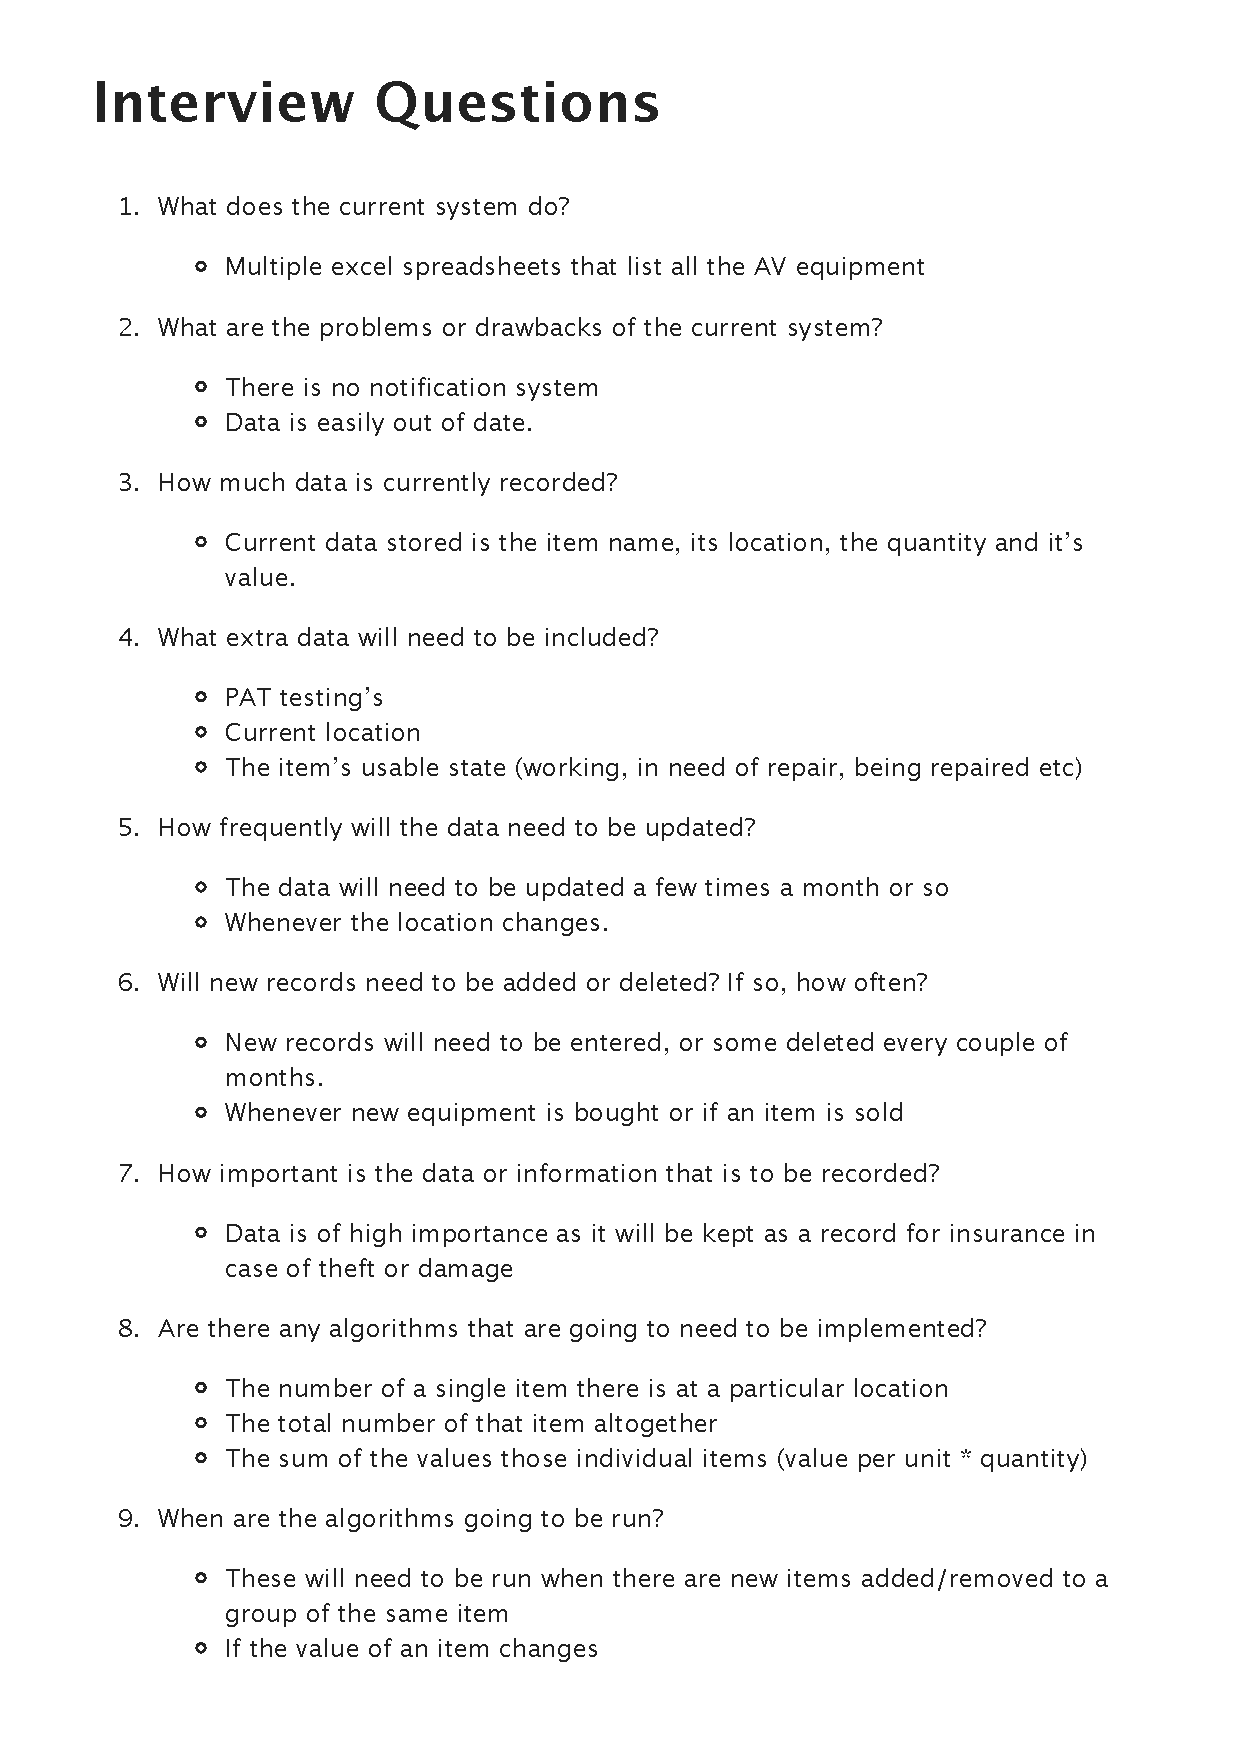
\includegraphics[page=1,width=\textwidth]{./Interview/interview_questions.pdf}
\end{figure}

\begin{figure}[H]
    \caption{Interview Questions (pg 2)} \label{fig: Interview Questions}
    \includegraphics[page=2,width=\textwidth]{./Interview/interview_questions.pdf}
\end{figure}

\begin{figure}[H]
    \caption{Interview Questions (pg 3)} \label{fig: Interview Questions}
    \includegraphics[page=3,width=\textwidth]{./Interview/interview_questions.pdf}
\end{figure}

\section{Investigation}

\subsection{The current system}

\subsubsection{Data sources and destinations}

In the current system, there are multiple data sources. The client and his colleagues as well as members of the AV crew for the church can enter data into the spreadsheet by using a computer in the office and accessing the on the server.

\subsubsection{Algorithms}

In the current system, there are only a few algorithms in place.
\bigskip

Algorithm 1, When new item is bought:
\begin{lstlisting}
IF Item = NewItem DO
        Enter Item into Spreadsheet
    ELIF Item = ItemMatch Do
        Update Item Quantity
\end{lstlisting}
\bigskip

Algorithm 2, When an item is sold or replaced:
\begin{lstlisting}
IF Item = Sold OR Item = Damaged or Item = Stolen DO
    Update Quantity
    IF Item = Stolen OR Item = Damaged DO
        Claim Insurance
\end{lstlisting}



\subsubsection{Data flow diagram (part 1)}

\begin{figure}[H]
    \caption{Flow Diagram Key.} \label{fig:print_function_result}
    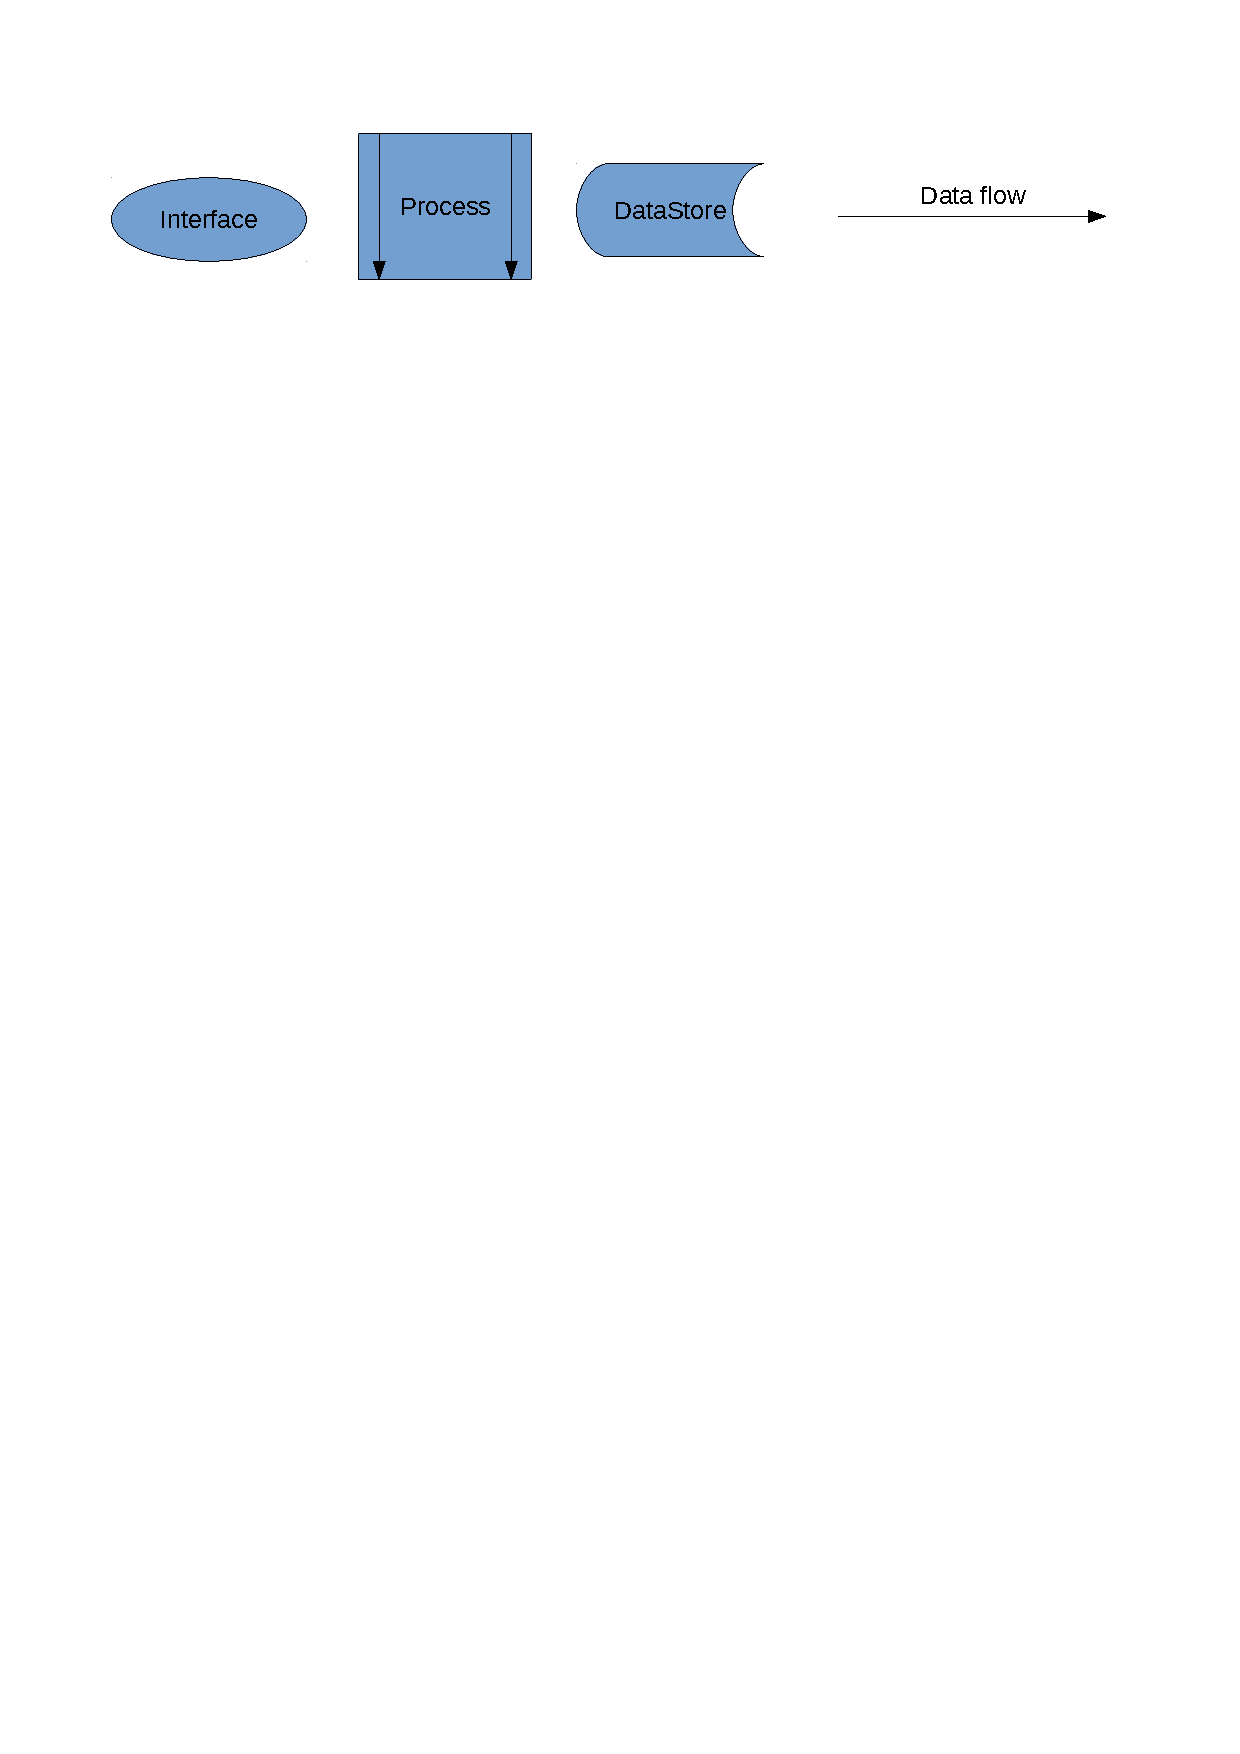
\includegraphics[width=\textwidth]{./DFD_analysis_key.pdf}
\end{figure}

\begin{figure}[H]
    \caption{Entering a new item.} \label{fig:print_function_result}
    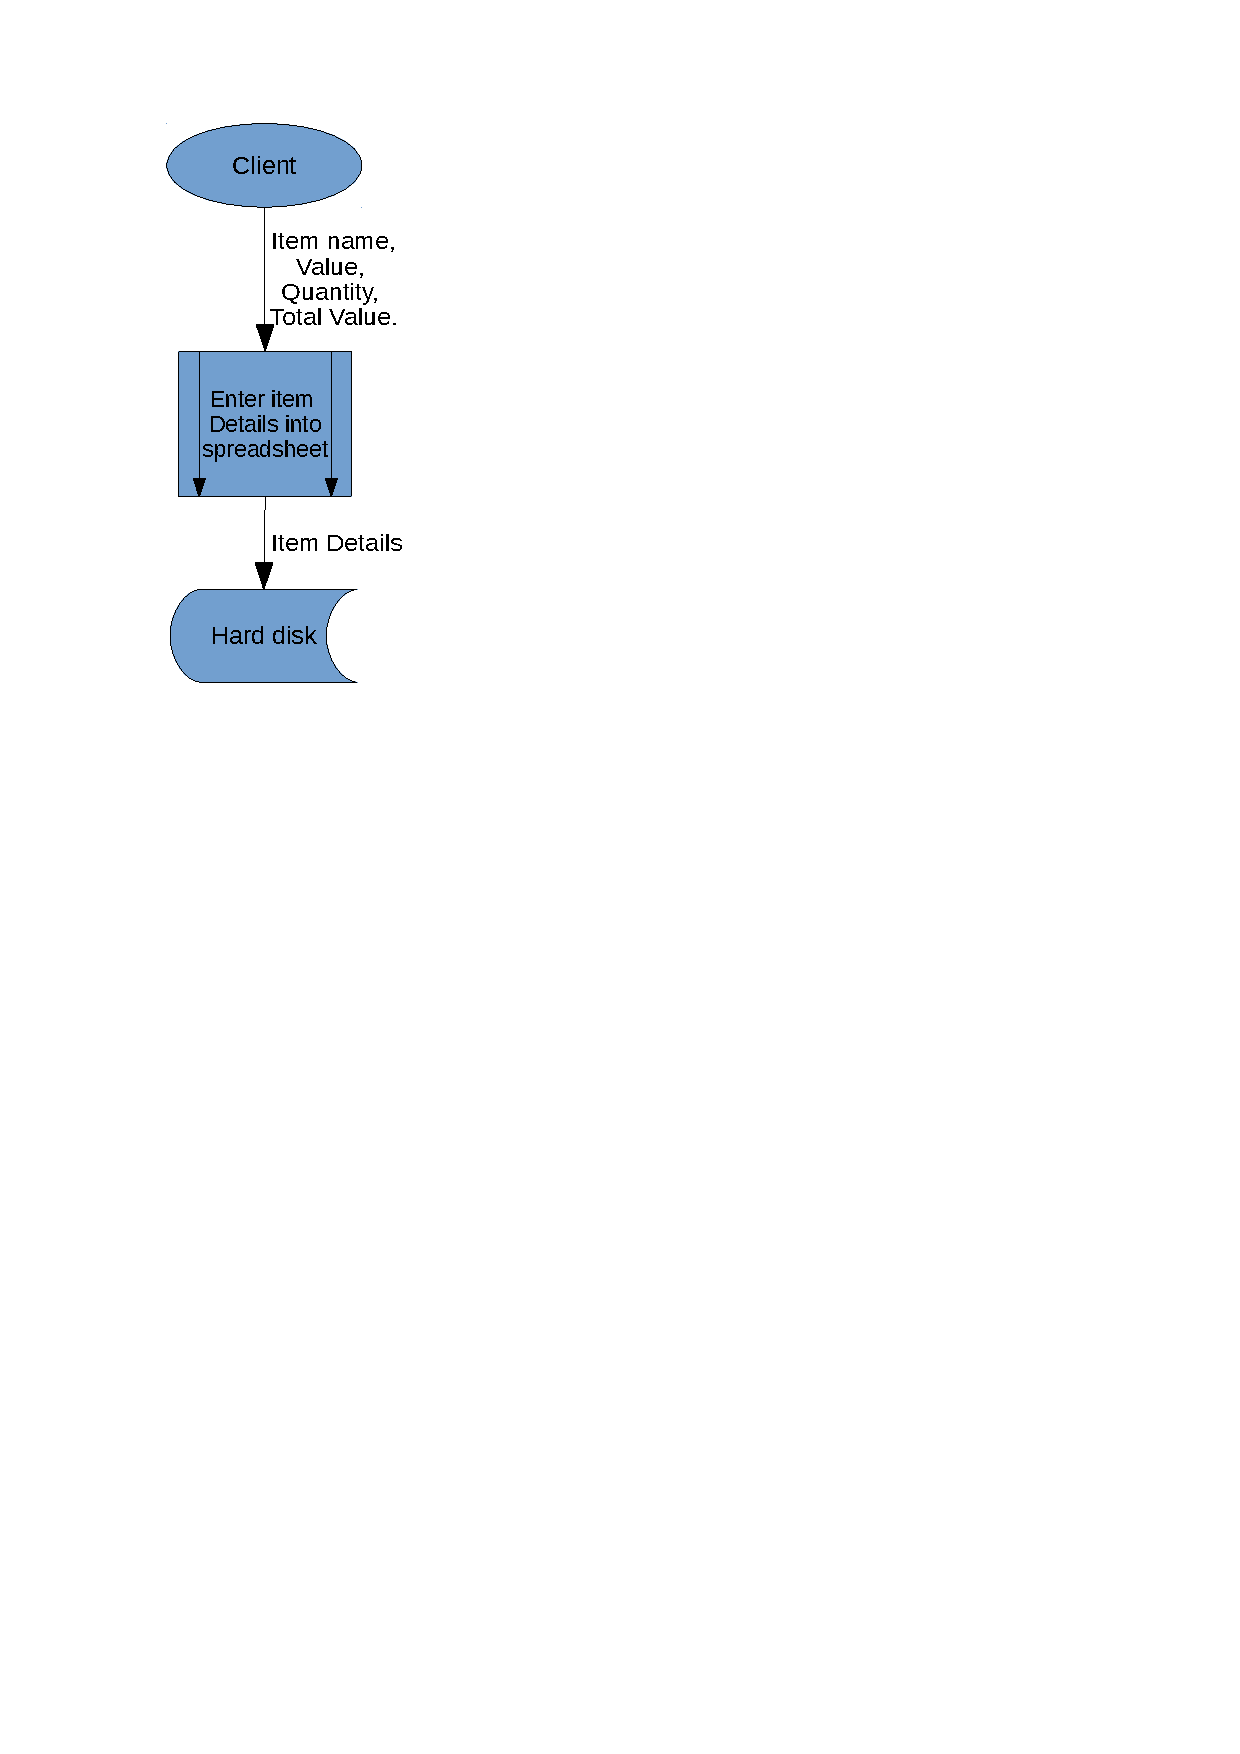
\includegraphics[width=50mm,scale=0.5]{./DFD_analysis_new_item.pdf}
\end{figure}

\newpage

\subsubsection{Data flow diagram (part 2)}

\begin{figure}[H]
    \caption{Flow Diagram Key.} \label{fig:print_function_result}
    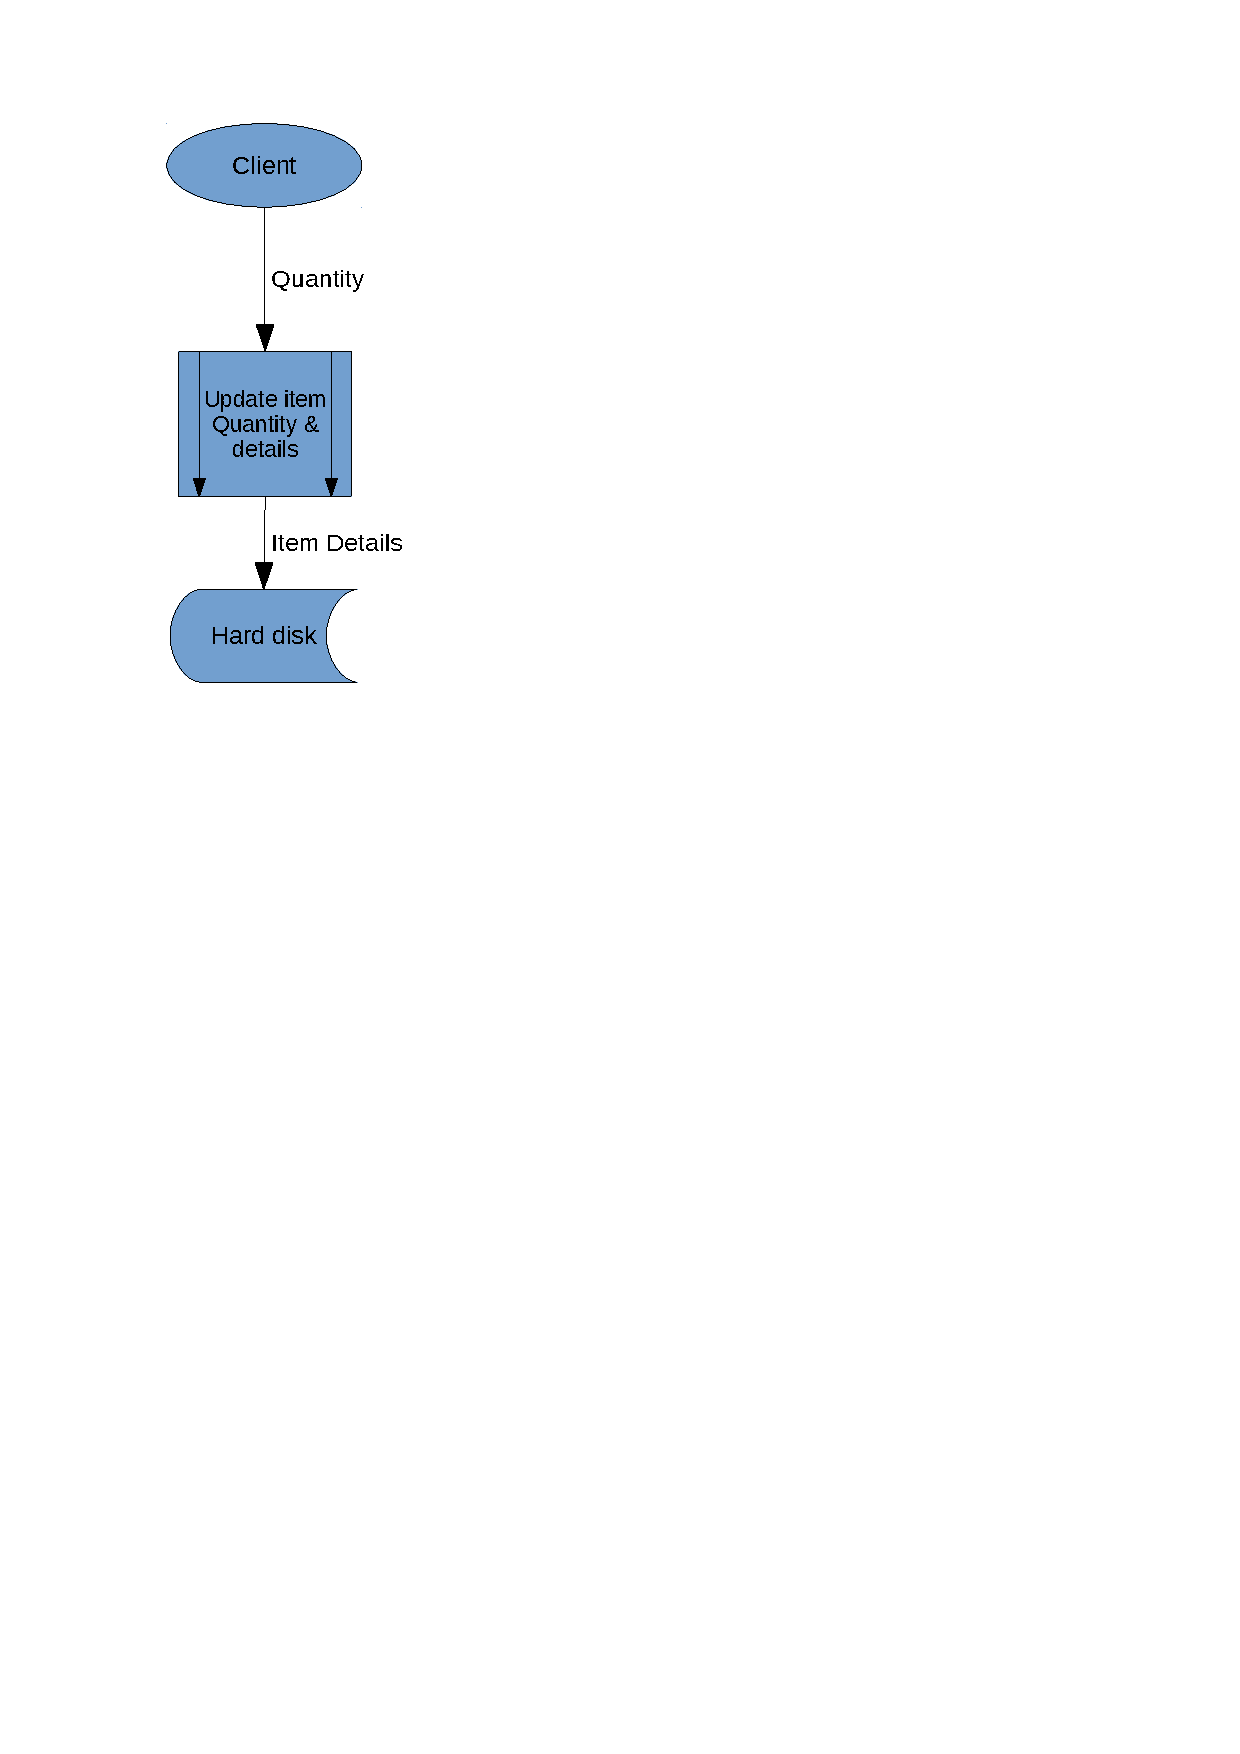
\includegraphics[width=50mm,scale=0.5]{./DFD_analysis_update_item.pdf}
\end{figure}

\newpage

\subsubsection{Input Forms, Output Forms, Report Formats}

Josh's current system only has one input form, this is the application excel. The system has 

\subsection{The proposed system}

\subsubsection{Data sources and destinations}

\subsubsection{Data flow diagram}

\subsubsection{Data dictionary}

\subsubsection{Volumetrics}

\section{Objectives}

\subsection{General Objectives}

\subsection{Specific Objectives}

\subsection{Core Objectives}

\subsection{Other Objectives}

\section{ER Diagrams and Descriptions}

\subsection{ER Diagram}

\subsection{Entity Descriptions}

\section{Object Analysis}

\subsection{Object Listing}

\subsection{Relationship diagrams}

\subsection{Class definitions}

\section{Other Abstractions and Graphs}

\section{Constraints}

\subsection{Hardware}

\subsection{Software}

\subsection{Time}

\subsection{User Knowledge}

\subsection{Access restrictions}

\section{Limitations}

\subsection{Areas which will not be included in computerisation}

\subsection{Areas considered for future computerisation}

\section{Solutions}

\subsection{Alternative solutions}

\subsection{Justification of chosen solution}

\end{document}